
 
\documentclass[12pt,letterpaper]{article}
 
%\usepackage{cvpr}
%\documentclass[11pt,letterpaper]{article}
\setlength{\textheight}{8.875in}
\setlength{\textwidth}{6.875in}
\setlength{\columnsep}{0.3125in}
\setlength{\topmargin}{0in}
\setlength{\headheight}{0in}
\setlength{\headsep}{0in}
\setlength{\parindent}{1pc}
\setlength{\oddsidemargin}{-.304in}
\setlength{\evensidemargin}{-.304in}
 
\usepackage{times}
\usepackage{bbm}
\usepackage{epsfig}
\usepackage{graphicx}
\usepackage{amsmath}
\usepackage{amssymb}
\usepackage{amsthm}
\usepackage{mathrsfs}
\usepackage{caption}
\usepackage{subcaption}
%\usepackage{caption}
\DeclareMathOperator*{\argmin}{\arg\!\min}
\newtheorem{lemma}{Lemma}
\newtheorem{proposition}{Proposition}
\newtheorem{theorem}{Theorem}
\newtheorem{coro}{Corollary}
\newtheorem{prop}{Property}
\newtheorem{definition}{Definition}
 
% If you comment hyperref and then uncomment it, you should delete
% egpaper.aux before re-running latex. (Or just hit 'q' on the first latex
% run, let it finish, and you should be clear).
 
 
 
\def\texte#1{#1}
 
\begin{document}
\def\RR{\mathbb{R}}
\def\PP{\mathbb{P}}
\def\AA{\mathbb{A}}
\def\LL{\mathbb{L}}
\def\SS{\mathbb{S}}
\def\barr{\bar{\mathbb{R}}}
\def\mat#1{{\mathcal{#1}}}
\def\vect#1{\mbox{\boldmath $#1$}}
\def\PPi{\mbox{\boldmath$\Pi$}}
\def\squig{\rightsquigarrow}
%\def\vect#1{#1}
%\def\mat#1{#1}
\def\comment#1{{}}
%\def\qmatrix#1{\left[\begin{array}{l}#1\end{array}\right]}
\def\qmatrix#1{\left[\begin{matrix}#1\end{matrix}\right]}
 
\title{Kernel Square-Loss Examplar Machines}
\author{Jean Ponce}
%\date{}
\maketitle
 
\begin{abstract}
Zepeda and P\'erez show in~\cite{ZePe15} that the weight vectors
associated with examplar SVMs can be used as global features
representing images in tasks such as retrieval or classification. A
drawback is the cost of the procedure, which requires a (convex)
optimization process to be run for each positive image. This note
shows that a more efficient approach can be obtained using a square
loss instead of the hinge loss. Building on~\cite{BaJo05,FiSc01}, it
also shows that this approach is easily kernelized, and, assuming
low-rank kernels, that the corresponding computational cost is linear
in the number of negative examples for each positive example. The
presentation concludes with a brief discussion of the relationship
between the proposed approach with linear discriminant analysis and
its use in region matching in~\cite{ARS14}.
\end{abstract}
 
 
\section{Square-loss examplar machines\label{sec:sqesvm}}
Given some loss function $L:[-1,+1]\times \RR\rightarrow \RR^+$, some
positive training example $x_0$ in $\RR^p$ and $n$ negative training
examples $x_i$ in $\RR^p$ ($i=1,\ldots,n$), training an exemplar
linear classifier consists in minimizing the error
\begin{equation}
E(w,b)=\frac{1}{n}\sum_{i=1}^n L(-1,w\cdot x_i+b)+ L(1,w\cdot
x_0+b)+\frac{\lambda}{2} ||w||^2
\label{eq:general}
\end{equation}
with respect to $w$ in $\RR^p$ and $b$ in $\RR$.
 
The traditional examplar SVM uses the hinge loss for $L$. Let us use
instead the square loss. Equation~(\ref{eq:general}) becomes
\begin{equation}
E(w,b)=\frac{1}{2n}\sum_{i=1}^n (w\cdot x_i+b+1)^2+ \frac{1}{2}(w\cdot
x_0+b-1)^2+\frac{\lambda}{2} ||w||^2.
\label{eq:square}
\end{equation}
 
The interest of the square loss is that the minimization can be done
in closed form. Indeed, writing that $\partial E/\partial b=0$ at a
minimum yields
\begin{equation}
b=-\frac{1}{2}(x_0+\mu)\cdot w,
\end{equation}
where $\mu=\frac{1}{n}\sum_{i=1}^n x_i$ is the center of mass of the
negative samples $x_i$.
 
Substituting in Eq.~(\ref{eq:square}) now reduces our optimization problem
to the minimization with respect to $w$ of
\begin{equation}
\begin{array}{lcl}\hat{E}(w)&=&
\displaystyle\frac{1}{2n}\sum_{i=1}^n [w\cdot (x_i-\frac{1}{2}(x_0+\mu))+1]^2
+\frac{1}{2}[w\cdot (x_0-\frac{1}{2}(x_0+\mu))-1]^2+\frac{\lambda}{2}||w||^2\\
&=&
\displaystyle\min_{w\in\RR^p}
\frac{1}{2n}\sum_{i=1}^n [w\cdot (\sigma_i-\frac{1}{2}\delta) +1]^2
+\frac{1}{2}(\frac{1}{2}w\cdot\delta-1)^2+\frac{\lambda}{2}||w||^2,
\end{array}
\label{eq:weq}
\end{equation}
where $\delta=x_0-\mu$ and $\sigma_i=x_i-\mu$.
 
Finally, writing $\partial\hat{E}/\partial w=0$ at a minimum yields
\begin{equation}
\frac{1}{n}\sum_{i=1}^n [w\cdot(\sigma_i-\frac{1}{2}\delta)+1](\sigma_i-\frac{1}{2}\delta)
+\frac{1}{2}(\frac{1}{2}w\cdot\delta-1)\delta +\lambda w=0,
\end{equation}
or
\begin{equation}
[\frac{1}{n}\sum_{i=1}^n(\sigma_i-\frac{1}{2}\delta)(\sigma_i^T-\frac{1}{2}\delta^T)] w
+\frac{1}{n}\sum_{i=1}^n (\sigma_i-\frac{1}{2}\delta) +\frac{1}{2}\delta\frac{1}{2}\delta^T w -\frac{1}{2}\delta +\lambda w
=0.
\end{equation}
 
Using the fact that the variables $\sigma_i$ have zero
mean, we obtain
\begin{equation}
[\frac{1}{n}\sum_{i=1}^n\sigma_i\sigma_i^T +\frac{1}{2}\delta\delta^T +\lambda\text{Id}]
w=\delta,
\end{equation}
or, putting everything together and reverting to the original notation,
\begin{equation}
\left\{\begin{array}{l}
\displaystyle w=A^{-1} (x_0-\mu),\quad\text{where}\quad
A=\Sigma
+\frac{1}{2}(x_0-\mu)(x_0-\mu)^T +\lambda\text{Id},\\
\displaystyle b=-\frac{1}{2}(x_0+\mu)\cdot w,
\end{array}\right.
\label{eq:final}
\end{equation}
where
\begin{equation}
\Sigma=\frac{1}{n}\sum_{i=1}^n(x_i-\mu)(x_i-\mu)^T
=\frac{1}{n}\sum_{i=1}^n x_ix_i^T-\mu\mu^T=\frac{1}{n}XX^T-\mu\mu^T,
\label{eq:Sigmadef}
\end{equation}
is the covariance matrix of the negative samples $x_i$, and
$X$ denotes the $p\times n$ matrix with columns $x_i^T$ ($i=1,\ldots,n$).
 
The vector $w$ (or the vector $[w;b]$) of this {\em square-loss
examplar machine} can potentially be used as a new representation for
the corresponding positive feature $x_0$. Note that this gives
asymmetric roles to positive and negative examples.
 
A similar approach (with no regularizer) is advocated for region
matching in~\cite{ARS14}. We will come back to this issue in the last
section of this presentation.
 
 
 
\section{Kernelized version}
Let us recall a few basic facts avout kernel methods for supervised
classification. We consider a reprodcing kernel Hilbert space (RKHS)
$H$ formed by real functions over some set
$X$, and denote by $k$ the corresponding reproducing kernel. We
address the following learning problem over $H\times\RR$:
\begin{equation}
\min_{h\in H,b\in\RR}
\sum_{i=1}^n L[y_i,h(x_i)+b] + \frac{\lambda}{2}||h||^2,
\label{eq:kernel}
\end{equation}
where the pairs $(x_i,y_i)$ ($i=1,\ldots,n$) in $X\times Y$ are
training samples, $Y=\RR$ (regression) or $Y=\{-1,1\}$
(classification), and $L: Y\times \RR\rightarrow\RR$ is some arbitrary
loss function. By definition of a reproducing kernel,
Eq.~(\ref{eq:kernel}) can be rewritten as
\begin{equation}
\min_{h\in H,b\in\RR}
\sum_{i=1}^n L[y_i,( \varphi(x_i)|h)+b] +
\frac{\lambda}{2}||h||^2,
\label{eq:kernelaff}
\end{equation}
where $\varphi$ is the {\em feature map} over $X$ associated with the
kernel $k$ (which may not admit a known explicit form). We dub
problems with the general form of (\ref{eq:kernelaff}) {\em affine}
supervised learning problems since, given some fixed element $h$ of
$H$ and some scalar $b$, $(h|h')+b$ is an affine function of $h'$,
whose zero set defines an affine hyperplane of $H$ considered itself
as an affine space.
 
 
Let $K$ denote the kernel matrix with entries $k_{ij}=[\varphi(x_i)|
\varphi(x_j)]$ and rows $k_i^T$ ($i=1,\ldots,n$). We assume from now
on that $L$ is convex and continuous. We have the following theorem.
 
\begin{theorem}\label{th:affinelearn}
Equation~(\ref{eq:kernelaff}) admits equivalent primal and dual
versions.
 
The primal problem is
\begin{equation}
\min_{\alpha\in\RR^n,b\in\RR} \sum_{i=1}^n L[y_i,k_i^T\alpha+b]
+\frac{\lambda}{2}\alpha^TK\alpha,
\label{eq:primal1}
\end{equation}
and any solution $(\alpha^\star,b^\star)$ to (\ref{eq:primal1})
provides
a solution $(h^\star,b^\star)$ to (\ref{eq:kernelaff}) with
$h^\star=\sum_{i=1}^n \alpha_i^\star\varphi(x_i)$.
 
Let $r$ denote the rank of the kernel matrix $K$, a
{\em reduced} version of the primal problem is
\begin{equation}
\min_{\beta\in\RR^r,b\in\RR} \sum_{i=1}^n L[y_i,b_i^T\beta+b]
+\frac{\lambda}{2}||\beta||^2,
\label{eq:primal2}
\end{equation}
where $B$ is the $n\times r$ square root of $K$ and $b_i^T$ denotes
its $i$th row,
and any solution $(\beta^\star,b^\star)$ to (\ref{eq:primal2})
provides
a solution $(h^\star,b^\star)$ to (\ref{eq:kernelaff}) with
$h^\star=\sum_{i=1}^n \alpha_i^\star\varphi(x_i)$, and
$\alpha^\star=P\beta^\star$, where $P$ is the pseudo-inverse of $B^T$.
 
The dual problem is
\begin{equation}
\min_{\alpha\in\RR^n}
\sum_{i=1}^n L^*(y_i,-\lambda\alpha_i)
+\frac{\lambda}{2}\alpha^TK\alpha
\quad\text{subject to}\quad \sum_{i=1}^n \alpha_i=0,
\label{eq:finaldual}
\end{equation}
and the optimal value $b^*$ of $b$ given any solution
$\alpha^\star$ of (\ref{eq:finaldual}) can be found by solving
\begin{equation}
\min_{b\in \RR} \sum_{i=1}^n L(y_i,k_i^T\alpha^{\star}+b).
\label{eq:minb}
\end{equation}
The pair $(\alpha^\star,b^\star)$ then provides a solution
$(h^\star,b^\star)$ to (\ref{eq:kernelaff}) with $h^\star=
\sum_{i=1}^n\alpha_i^\star\varphi(x_i)$.
\end{theorem}
 
Note that, given a solution $(\alpha^\star,b^\star)$ of either the
primal or the dual version of (\ref{eq:kernelaff}), the optimal
prediction function is
\begin{equation}
[h^\star|\varphi(x)]+b^\star= \sum_{i=1}^n \alpha_i^{\star} K(x,x_i) +b^\star.
\end{equation}
 
Theorem\ref{th:affinelearn} follows fromt the representer theorem
~\cite{SHS01,Wahba90} and elementary results from analysis and
optimization theory.
 
In our context, the reduced primal version of Theorem 1 is
particularly interesting since the results of Section~\ref{sec:sqesvm}
directly apply to it: One simply has to replace $x_0$ and $\mu$ in
Eq.~(\ref{eq:final}) by appropriate columns of $B^T$, or linear
combinations thereof (in this case of course, the kernel matrix has
dimension $(n+1\times n+1)$). It is of course not clear whether the
corresponding vector $w$ would prove useful as a feature for
classification or other tasks.
 
The next section shows how to train the kernel square-loss examplar
machine efficiently.
 
 
 
\section{Efficient implementation}
Let us consider the $n\times n$ kernel matrix $\hat{K}$ associated with
the $n$ negative examples, and a low-rank factorization $\hat{K}=\hat{B}\hat{B}^T$
of
this matrix, where $\hat{B}$ is an
$n\times r$ square root of $\hat{K}$. This factorization can be computed in $O(nr^2)$ time
and $O(nr)$ storage~\cite{BaJo05,FiSc01}. The singular value
decomposition $UWV^T$ of $\hat{B}$ and its $r\times n$ pseudoinverse
$\hat{B}^\dagger=(\hat{B}^T\hat{B})^{-1}\hat{B}^T=VW^{-1}U^T$ such that $\hat{B}^\dagger
\hat{B}=\text{Id}$ can also be computed with the same time and storage
costs.
 
Let us consider the augmented
kernel matrix $K$ obtained by adding one more (positive) sample. This matrix
can be written as
\begin{equation}
K=\qmatrix{k_{00} & k_0^T\\k_0& \hat{K}},
\end{equation}
where $k_{00}$ is a scalar and $k_0$ is an element of $\RR^n$.
The following
lemma show that a $(n+1)\times (r+1)$ factorization of $K$ can
be computed efficiently as well.
 
\begin{lemma}
The augmented kernel matrix $\hat{K}$ can be factorized as
\begin{equation}
\hat{K}=BB^T,\quad\text{where}\quad
B=\qmatrix{u & v^T\\0 & \hat{B}}\quad\text{and}\quad
v=\hat{B}^\dagger k_0,\,\, u=\sqrt{k_{00}-||v||^2}
\end{equation}
in time $O(nr)$ and storage $O(n)$.
\end{lemma}
\begin{proof}
Indeed,
\begin{equation}
BB^T=\qmatrix{u^2+||v||^2 & v^T\hat{B}^T\\ \hat{B}v & \hat{B}\hat{B}^T}.
\end{equation}
Since $K$ is positive semidefinite $k_0$ must lie in the column space
$\cal \hat{B}$ of $\hat{B}$,\footnote{Let
us assume that $k_0$ does not belong to $\cal \hat{B}$, then it can be
decomposed uniquely as $k_0=l_0+m_0$, where $l_0$ belongs to $\cal \hat{B}$,
and $m_0\neq 0$ belong to the orthogonal complement $\cal \hat{B}^\perp$ of
$\cal \hat{B}$. Obviously $(1,-\nu m_0^T)K(1;-\nu m_0)=k_{00}-2\nu||m_0||^2$, which
is negative for large enough values of $\nu>0$. In turn, this contradicts the
fact that a kernel matrix is positive semidefinite.}
and $b=\hat{B}^\dagger k_0$ is thus an exact solution of
$\hat{B}b=k_0$.
The fact that $k_{00}-||b||^2$ is nonnegative follows immediately from
the fact that the Schur complement $\hat{K}-||k_0||^2/k_{00}$ of $k_{00}$ in
the positive semidefinite matrix $K$ is itself positive semidefinite.\footnote{Indeed,
since the matrix $k_{00}K-k_0k_0^T=\hat{B}(k_{00}\text{Id}-bb^T)\hat{B}^T$ is
positive semidefinite, and $\hat{B}$ has rank $r$, the $r\times r$ matrix
$k_{00}\text{Id}-bb^T$
is also positive definite, thus
$b^T(k_{00}\text{Id}-bb^T)b=||b||^2(k_{00}-||b||^2)\ge 0$.} The
cost of the factorization is dominated by the $O(nr)$ computation and $O(n)$ storage
of $b$
\end{proof}
 
Training the kernel square-loss examplar machine given $\hat{B}$ amounts to
computing
$\Sigma$ in (\ref{eq:Sigmadef}) and solving the $(r+1)\times (r+1)$
linear system in (\ref{eq:final}). Note that, because of the
particular structure of $B$, only one term in the sum in (\ref{eq:Sigmadef})
must be recomputed for each new positive example, with $O(r^2)$ cost.
The linear system itself can be solved in $O(r^3)$ cost.
 
Once the optimal parameters $\beta^\star$ haven been found, they can
be used directly as some representation of the positive example. The
corresponding value $\alpha^\star$ (or more correctly, {\em a}
corresponding value) can be computed as $\alpha^\star =P\beta^\star$,
where $P=B(B^TB)^{-1}$ is the pseudoinverse of $B^T$ with
$B^TP=\text{Id}$. The corresponding element of $\cal H$ is
$h^\star=\sum_{i=0}^n \alpha_i^\star\varphi(x_i)$.
 
Now, given two positive images $x_0$ and $x_0'$, they can be compared
by computing the normalized inner product
\begin{equation}
s(x_0,x_0')=\frac{(h|h')}{\sqrt{(h|h)}\sqrt{(h'|h')}}
\end{equation}
of the corresponding elements $h$ and $h'$ of $H$ as a similarity measure
(we drop the ``$\star$'' exponents from now on to avoid clutter in the
noration).
 
Concretely, we have
\begin{equation}
\begin{array}{lcl}
(h|h')&=&\displaystyle[\alpha_0\varphi(x_0)+\sum_{i=1}^n\alpha_i\varphi(x_i)
|\alpha_0'\varphi(x_0')+\sum_{i=1}^n\alpha_i'\varphi(x_i)]\\
&=&\displaystyle
\alpha_0\alpha_0'\displaystyle k(x_0,x_0')+ \alpha_0\sum_{i=1}^n\alpha_i' k(x_0,x_i)
+\alpha_0'\sum_{i=1}^n
\alpha_ik(x_0',x_i)+\hat{\alpha}^T\hat{K}\hat{\alpha}'\\
&=&\displaystyle\alpha_0\alpha_0'\displaystyle k(x_0,x_0')+ \alpha_0k_0^T\hat{\alpha}'
+\alpha_0'k_0'^T\hat{\alpha}
+\hat{\alpha}^T\hat{K}\hat{\alpha}'\\
\end{array}
\label{eq:lcl}
\end{equation}
where $\hat{\alpha}$ (resp. $\hat{\alpha}'$) denotes the vector of
$\RR^n$ formed by excluding the first (or rather zeroth) element
of $\alpha$ (resp. $\alpha'$).
 
 
 
If we write $\beta = [\beta_0; \hat{\beta}]$ similarly to
$\alpha=[\alpha_0; \hat{\alpha}]$ and keeping in mind that
$P=[\frac{1}{u}\ 0; -\frac{1}{u}\hat{P}v \ \hat{P}]$, where $\hat{P}$
is the pseudoinverse of
$\hat{B}^T$, we have that
\begin{equation}
\alpha_0 = \dfrac{\beta_0}{u}, \,\, \hat{\alpha}=-\dfrac{\beta_0}{u}Pv+P\hat{\beta}.
\end{equation}
Remembering that $\hat{K}=\hat{B}\hat{B}^T$ and and $k_0=\hat{B}v$
allows us to rewrite (\ref{eq:lcl}) as
\begin{align}
(h|h')& = \dfrac{\beta_0\beta_0'}{uu'}k(x_0,x_0')
+\dfrac{\beta_0}{u}v^T\hat{B}^T\left(-\dfrac{\beta_0'}{u'}Pv'+P\hat{\beta'}\right)
+\dfrac{\beta_0'}{u'}v'^T\hat{B}^T\left(-\dfrac{\beta_0}{u}Pv+P\hat{\beta}\right)\\ &+\left(\hat{B}^T\left(-\dfrac{\beta_0}{u}Pv+P\hat{\beta}\right)\right)^T
\left(\hat{B}^T\left(-\dfrac{\beta_0'}{u'}Pv'+P\hat{\beta'}\right)\right)\\ &=
\dfrac{\beta_0\beta_0'}{uu'}k(x_0,x_0')
+\dfrac{\beta_0}{u}v^T\left(-\dfrac{\beta_0'}{u'}v'+\hat{\beta'}\right)
+\dfrac{\beta_0'}{u'}v'^T\left(-\dfrac{\beta_0}{u}v+\hat{\beta}\right)
+
\left(-\dfrac{\beta_0}{u}v+\hat{\beta}\right)^T\left(-\dfrac{\beta_0'}{u'}v'+\hat{\beta'}\right)\\ &=
\hat{\beta}^T\hat{\beta'}
+\dfrac{\beta_0\beta_0'}{uu'}\left(k(x_0,x_0')-v^Tv'\right).
\end{align}
We also note that $(h|h)=||\beta||^2$ and $(h'|h')=||\beta'||^2$.

Furthermore, from the solution of the linear system (\ref{eq:final}), we find that $\beta_0 = \frac{cu}{\lambda}$, $\hat{\beta} = cG^{-1}(v-\mu)$ and $\beta_0' = \frac{cu'}{\lambda}$, $\hat{\beta}' = c'G^{-1}(v'-\mu)$, for $c,\ c'$ scalars and $G = \frac{1}{n}\hat{B}^T\hat{B}-\mu\mu^T+\lambda\text{Id}$. The final similarity score can be computed by
\begin{equation}
s(x_0,x_0') = \dfrac{(v-\mu)^TG^{-2}(v'-\mu)+\dfrac{1}{\lambda^2}(k(x_0,x_0')-v^Tv')}{\sqrt{(v-\mu)^TG^{-2}(v-\mu)+\dfrac{u^2}{\lambda^2}}\sqrt{(v'-\mu)^TG^{-2}(v'-\mu)+\dfrac{u'^2}{\lambda^2}}}
\end{equation}
 
\section{Notes: LDA and square-loss linear classifiers}
Let us now go back to linear classifiers, and suppose that we have
multiple positive samples. It is easy to show that in this case, the
corresponding linear classifier for the square loss is also given by
Eq.~(\ref{eq:final}), where $x_0$ denotes this time the center of mass
of the positive samples, {\em if} these samples have the {\em same}
covariance matrix $\Sigma$ as the negative ones.
 
This equal-covariance assumption is of course quite restrictive, and
probably unrealistic in general. It is interesting to note, however,
that this is exactly the assumption made by linear discriminant
analysis. As shown in~\cite{Hastie2009} for example, LDA can be seen as a
(non-regularized) linear classifier
with decision function $w'\cdot z+ b'$, where $z$ is a sample in
$\RR^p$, and
\begin{equation}
\left\{\begin{array}{l}
\displaystyle w'=\Sigma^{-1}(x_0-\mu),\\
\displaystyle b'=-\frac{1}{2}(x_0+\mu)\cdot w',
\end{array}\right.
\label{eq:lda}
\end{equation}
 
Note that when $\lambda=0$ (no regularization),
\begin{equation}
\Sigma w = Aw -\frac{1}{2}[(x_0-\mu)\cdot w] (x_0-\mu) =
[1-\frac{1}{2}(x_0-\mu)\cdot w](x_0-\mu)
=[1-\frac{1}{2}(x_0-\mu)\cdot w]\Sigma w'
\end{equation}
thus $w$ and $w'$ have the same direction. In other words, a
square-loss linear classifier is strictly equivalent to LDA when the
regularizer parameter $\lambda $ is zero.
 
More generally, as shown in~\cite{Hastie2009},
\begin{enumerate}
\item LDA is a nearest-centroid binary classifier using the
Mahalanobis distance under the assumption that the two classes
have the same covariance.
\item Its decision function is a Bayes classification rule for normal
distributions with different means but identical covariance matrices
when, in addition, the priors over the two classes are assumed to be
equal (the log-ratio of the prior probabilities must be added to the
offset otherwise). \footnote{In general, Hastie
{\em et al.}~recommend taking the priors $\pi_i$ equal to the proportion of points
in class $i$ among all points, that is the class with most samples is
most probable.}
\end{enumerate}
 
Once again, these facts are well known, but may be relevant (or not)
given recent renewed interest in LDA in modern classification
tasks~\cite{GMPD12,HMR12}, where some of these properties have been
rediscovered. In particular, as noted earlier, (non-regularized)
linear square-loss exemplar machines are proposed in~\cite{ARS14} as a
means to treat region matching as a classification problem. Aubry {\em
et al.} note in~\cite{ARS14} that the decision hyperplanes obtained by
this method and LDA are parallel (our analysis shows they are actually
identical --- there must be a mistake somewhere). They further show
that LDA scores calibrated using an additive constant give much better
results in their matching task. This is a bit puzzling since they
should give exactly the same results (same rankings and same scores up
to an affine transformation---before squaring the error term) for a
given positive example. Aubry {\em et al.} may mean calibration across
different positive examples. This needs to be clarified and perhaps
justified as well.
 
\section{SLEM versus whitening}
Due to Woodbury identity, Equation \ref{eq:final} can be rewritten as 
\begin{equation}
w = \Sigma^{-1}(x_0-\mu).
\end{equation}
In the original E-SVM work, the score of similarity between a query image $x_0$ and a possible result $x_0'$ is given by
\begin{equation}
s(x_0,x_0') = x_0'^T\Sigma^{-1}(x_0-\mu). \label{white:score}
\end{equation}
 
Under the assumption centered data and positive and negative data having the same covariance matrix (as proposed in the previous section), Equation \ref{white:score} corresponds to the score of whitened data:
\begin{align}
\hat{x_0} = \Sigma^{-\frac{1}{2}}(x_0-mu);\\
s(x_0,x_0') = \hat{x_0}^T\hat{x_0'}.
\end{align}
This observation has already been made by \cite{Koba15}. However, the score of similarity used in \cite{ZePe15} is
\begin{equation}
s(x_0,x_0') = (x_0'-\mu)^T\Sigma^{-2}(x_0-\mu). \label{esvm:score}
\end{equation}

Based on this, we propose the score $s_{\alpha}$ given by $s_{\alpha}(x_0,x_0') = (x_0-\mu)^T\Sigma^{\alpha}(x_0-\mu).$ $s_{-2}$ is the SLEM similarity score, $s_{-1}$ is the whitening similarity score and $s_{0}$ is the centered base features similarity score.

Strangely, both scores seem to perform similarly, even if their scores differ. Doing a singular value decomposition of $\Sigma$, $\Sigma^{-1}=VD^{-1}V^T$ and $\Sigma^{-\alpha}=VD^{-\alpha}V^T$.

\begin{figure}[!h]
\centering
\begin{subfigure}[b]{0.45\textwidth}
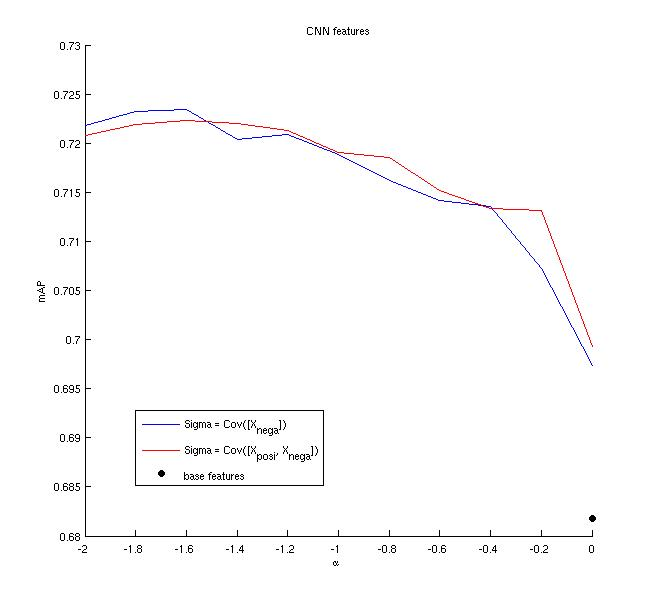
\includegraphics[width=\textwidth]{whitening_cnn.jpg}
\end{subfigure}
\begin{subfigure}[b]{0.45\textwidth}
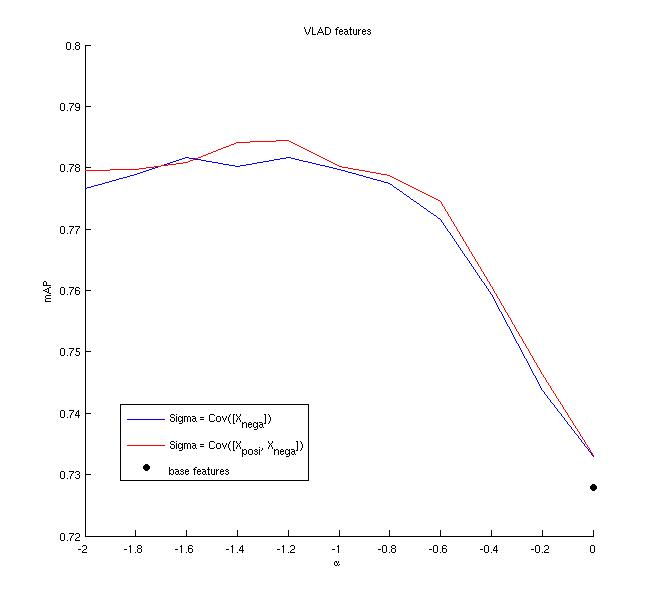
\includegraphics[width=\textwidth]{whitening_vlad.jpg}
\end{subfigure}
\caption{Comparison of mAP for different similarity scores $s_{\alpha}$, varying $\alpha$. At left, CNN features. At right, VLAD features. On blue, $\Sigma$ is the covariance of the negative samples and on red, $\Sigma$ is the covariance of the positive and negative samples. On black, the mAP for similarity calculated as inner product of base features.}
\label{Sigma}
\end{figure}

\section{Experiment Evaluation}
\subsection{Base image encoding}
We use three base features as the representation in $\RR^p$ of our images. The two firsts are VLAD and CNN features, as used in \cite{ZePe15}. 
CNN features are non-negative and can be used both as $\mathbb{L}^1$ or $\mathbb{L}^2$ normalized features. The third features are pyramids of histograms of SIFT descriptors, as used in \cite{spk}. These are non-negative $\mathbb{L}^1$ normalized features.

\subsection{Kernels}
For all features, we test non-kernelized SLEM, as well as kernelized SLEM for gaussian (rbf) and polynomial kernel:
\begin{align}
k_{rbf}(x,y) &= \exp\left(-\gamma||x-y||^2\right);\\
k_{poly}(x,y) &= x^Ty+\gamma(x^Ty)^2.
\end{align}
For non-negative $\mathbb{L}^1$ normalized, we also test the intersection kernel: $k_{inter}(x,y) = \min(x,y).$\\
We observe that the non-kernelized obtains similar results to kernels polynomial and Gaussian. For the pyramid histogram of SIFT, the intersection kernel works much better than all the other kernels.

\begin{table}
\begin{center}
\begin{tabular}{|l|c|c|c|c|}
\hline
Method & $s_0$ & $s_{-2}$ with no kernel & $s_{-2}$ for gaussian kernel &  $s_{-2}$ for intersection kernel \\
\hline\hline
VLAD-64 & 73.3 & 77.9 & 78.1 & -\\
Caffe CNN & 69.7 & 72.1 & 72.9 & 70.2\\
Pyramid of Histogram & 38.7 & 43 & 44.6 & 63.5\\
\hline
\end{tabular}
\end{center}
\caption{Results.}
\end{table}

\bibliographystyle{plain}
\bibliography{sup}
\end{document}
 
 
